\documentclass[11pt,a4paper]{article}
\usepackage[utf8]{inputenc}
\usepackage[T1]{fontenc}
\usepackage{graphicx}
\usepackage{booktabs}
\usepackage{float}
\usepackage[section]{placeins}
\usepackage[margin=2.5cm]{geometry}
\usepackage[hidelinks,breaklinks]{hyperref}
\usepackage{amsmath}
\usepackage{enumitem}
\usepackage{setspace}
\usepackage{xurl}
\usepackage[labelfont=bf]{caption}
\usepackage{xcolor}
% Changes from earlier rounds are no longer highlighted; third-round (R3)
% changes are shown in red via \rthree{}.
\newcommand{\revised}[1]{#1}
\newcommand{\rtwo}[1]{#1}
\newcommand{\rthree}[1]{#1}
\onehalfspacing

\title{\LARGE\bfseries \rtwo{Leakage-Free Evaluation of Layer Choice in Protein Language Models for Mutation Effect Prediction}}

\author{
\large
Yutao Guo\textsuperscript{1,2}, Zihan Zhang\textsuperscript{1,2}, Xuezhou Zhao\textsuperscript{1,2},\\[2pt]
Mengxi Chen\textsuperscript{1,2}, Dan Wu\textsuperscript{1,3*}\\[8pt]
\small
\textsuperscript{1}International College of Pharmaceutical Innovation,\\
\hspace*{1em}Soochow University, Suzhou 215123, China\\[4pt]
\textsuperscript{2}School of Pharmacy and Biomolecular Sciences, RCSI,\\
\hspace*{1em}123 St Stephen's Green, Dublin 2, D02 VN51, Ireland\\[4pt]
\textsuperscript{3}Department of Chemistry, RCSI,\\
\hspace*{1em}123 St Stephen's Green, Dublin 2, D02 YN77, Ireland\\[8pt]
*Corresponding author: \texttt{danwu@suda.edu.cn}}
\date{}

\begin{document}
\maketitle

\begin{abstract}
\textbf{Motivation:} \rtwo{Multi-layer embedding fusion is widely used with protein
language models (PLMs) such as ESM-2, on the assumption that different layers carry
complementary mutation-relevant information. This assumption has not been tested
systematically for mutation effect prediction.}

\textbf{Results:} \rtwo{We benchmarked ESM-2 and the structure-aware SaProt (650M
parameters each) on 63 ProteinGym substitution assays using per-layer probing under
four train--test splits, multi-scale pooling, a logit lens, and a position-lookup
control. Under the standard random split all 33 layers performed alike
($\rho \approx 0.60$), but random position vectors reproduced this level and collapsed
to $0.10$--$0.14$ under leakage-free splits: random-split layer interchangeability is a
property of the evaluation, not of the representations. Under leakage-free splits,
performance rose with depth (ESM-2: $\rho = 0.23$ at layer 0, $0.46$ at layer 32), and
the best layer (layers 27--32) exceeded the final layer by at most
\rthree{$\Delta\rho = 0.019$ (90\% upper bound $0.036$). This deficit is small relative
to the cross-dataset standard deviation of $0.17$. Multi-scale pooling did not reliably
improve on the final layer under leakage-free evaluation (1 of 96 comparisons
significantly better, 55 worse), whereas fusion gains appeared under the random
split.} Real 3Di structure tokens improved
SaProt slightly under the random split and substantially under leakage-free splits
(\rthree{$+0.06$ to $+0.13$}). A validated logit lens peaked at the final layer and reproduced
published ProteinGym zero-shot scores on single-substitution assays. Depth matters,
and the final layer is a sufficient choice.}

\textbf{Availability and Implementation:} \rtwo{Code and per-dataset results are
available at \url{https://github.com/schwarzeteeguo-creator/esm2-layer-invariance} and
archived at Zenodo (DOI: 10.5281/zenodo.22844290).}
\end{abstract}

%=============================================================================
\section{Introduction}
%=============================================================================

Protein language models (PLMs) pre-trained via masked language modeling (MLM) on
millions of protein sequences have become indispensable for mutation effect
prediction~\cite{rives2021biological,meier2021language,lin2023evolutionary}.
Among these, ESM-2~\cite{lin2023evolutionary}
is one of the most widely adopted, with a 650M-parameter architecture comprising 33
transformer layers that produce 1280-dimensional per-residue hidden states. These
embeddings have been successfully applied to diverse tasks including variant effect
prediction~\cite{frazer2021disease,hie2021learning}, protein design, and functional
annotation~\cite{elnaggar2022prottrans,brandes2022proteinbert}, establishing ESM-2 as a
foundational tool in computational biology.

The internal organization of information across transformer layers has been
extensively studied in natural language processing, where the ``BERTology''
literature has revealed that different layers specialize
in distinct linguistic phenomena: lower layers encode surface-level syntax, middle
layers capture semantic content, and final layers refine task-specific
predictions~\rtwo{\cite{rogers2021bertology,tenney2019bert}}.
This hierarchical view has motivated analogous investigations in protein language
models. A growing body of work posits that different transformer layers in PLMs
similarly encode complementary biochemical information, and that combining
representations from multiple layers should therefore improve downstream tasks.
Kumar and Jha~\cite{kumar2025} demonstrated that mid-to-late ESM-2 layers (20--33)
outperform the final layer for kinase function prediction, while early layers
(6--14) have been shown to encode local physicochemical properties such as
hydrophobicity and secondary structure propensity~\cite{detlefsen2022}.
Alsamkary, Elshaffei et al.~\cite{elshaffei2025} proposed hierarchical pooling and
pooled attention architectures for fusing representations across multiple PLMs and
reported up to a 12\% Spearman improvement for protein--protein interaction
prediction. More broadly, the strategy of extracting and fusing embeddings from
multiple transformer layers\rtwo{, or from multiple PLMs~\cite{ko2026fusion,si2024contact},} has
become common practice in PLM-based pipelines~\cite{rao2019tape}, often under the
implicit assumption that each \rtwo{source} contributes non-redundant information.

These claims, however, rest on an assumption that has not been systematically tested:
that different ESM-2 layers genuinely encode \emph{complementary} information for
mutation effect prediction, rather than merely offering different views of the same
underlying signal. If layers are functionally similar under a given readout and
evaluation protocol, then multi-scale fusion may add cost without improving prediction.
If layer complementarity appears only under specific readouts or split protocols,
then layer selection should be treated as a conditional design choice rather than
a universal rule. Resolving this question carries practical
consequences: the computational cost of extracting and storing embeddings from
multiple layers is substantial for large-scale screening efforts, and the
proliferation of ad-hoc layer-selection heuristics complicates reproducibility.

To resolve this question, we conducted a large-scale benchmark on ProteinGym~\cite{notin2024proteingym},
a comprehensive collection of deep mutational scanning (DMS) experiments spanning
diverse protein families, assay types, and organismal contexts. We employed
three independent experimental paradigms (Figure~\ref{fig:concept}): (1) per-layer supervised probing via Ridge
regression, (2) multi-scale embedding pooling with controlled feature sets, and
(3) logit lens zero-shot scoring. In parallel, we quantified layer-wise representational
similarity through cosine similarity \rtwo{and CKA} analysis. \rtwo{Together, these
approaches ask how much mutation-relevant information each layer carries, how it
changes with depth, and how the answer depends on the evaluation protocol. We find
that the random-split layer profile is largely position memorization, whereas
leakage-free evaluation shows that predictive information rises with depth, that the
final layer is a sufficient choice, and that structure tokens carry a measurable
benefit that the standard protocol largely hides.}

\begin{figure}[ht]
\centering
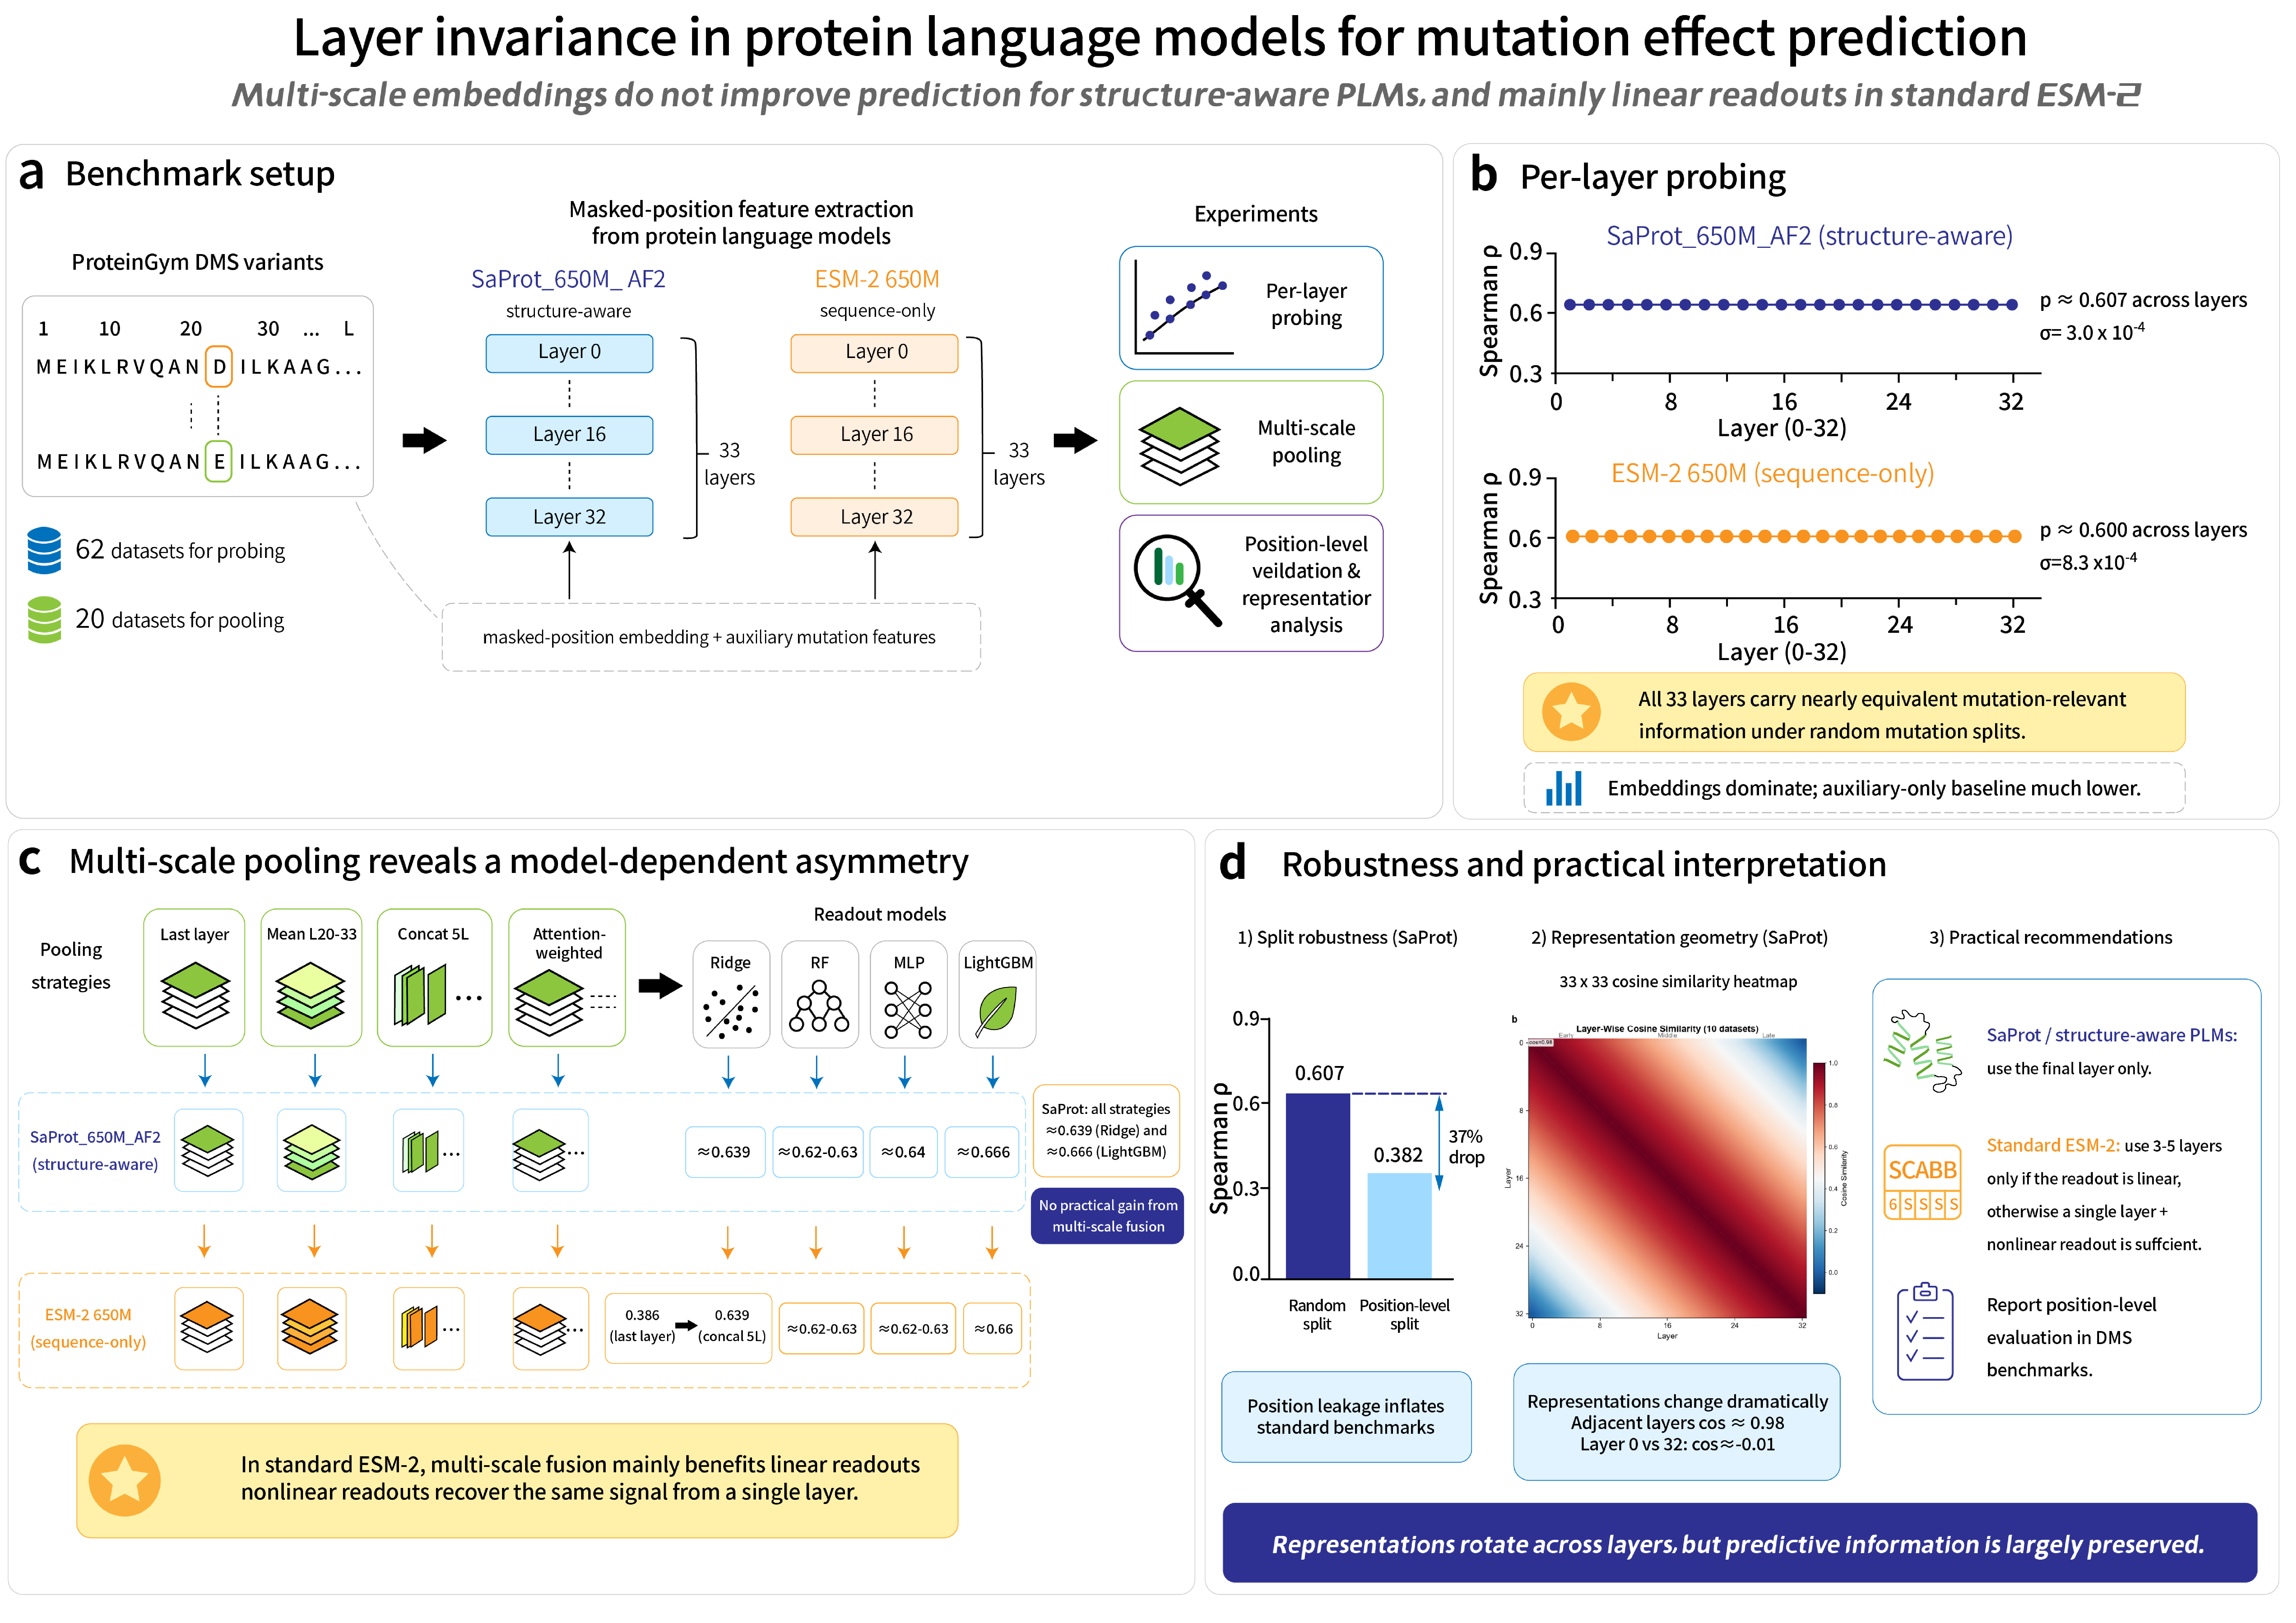
\includegraphics[width=\textwidth]{figures/output_r3/fig0_concept.pdf}
\caption{\textbf{Experimental design overview.}
The three complementary experimental paradigms employed in this study:
(\textbf{a}) Per-layer probing: Ridge regression on hidden states extracted from each
of the 33 transformer layers \revised{under three feature arms (masked wild-type,
unmasked wild-type, and mutant) and four train--test splits (random, modulo,
contiguous, and position-grouped), quantifying the predictive information content per
layer together with a random-position lookup control}.
(\textbf{b}) Multi-scale pooling: four embedding fusion strategies (Last Layer,
Mean L20--33, Concat 5L, Attention-weighted\revised{, with attention weights trained
within each cross-validation fold}) tested across four readout models
(Ridge, Random Forest, MLP, LightGBM) to assess whether combining layers improves
prediction.
(\textbf{c}) Logit lens: applying the final-layer LM head to intermediate hidden
states for zero-shot mutation scoring, directly measuring how token predictions
are refined across depth.
(\textbf{d}) Layer-wise cosine similarity analysis: quantifying representational
divergence independent of predictive performance.
\rtwo{Together, these paradigms measure how mutation-relevant information is
distributed across depth and whether combining layers adds to the final layer.}}
\label{fig:concept}
\smallskip{\footnotesize\rthree{\textit{Alt text:} Four-panel schematic of the study design: per-layer probing under three feature arms and four train--test splits with a position-lookup control (a), multi-scale pooling with four fusion strategies and four readouts (b), the logit lens (c), and layer-wise similarity analysis (d).}}
\end{figure}

%=============================================================================
\section{Methods}
%=============================================================================

\subsection{Models and Data}

We used SaProt\_650M\_AF2~\cite{su2024saprot}, a structure-aware variant of ESM-2 650M
that extends the vocabulary to 446 structure-informed tokens (21 amino acids $\times$ 21
Foldseek 3Di states~\cite{vankempen2024foldseek}), as our primary model. For validation,
we also tested standard ESM-2 650M~\cite{lin2023evolutionary} in both the probing and
logit lens experiments, enabling direct comparison between structure-aware and
sequence-only representations. All experiments used ProteinGym's substitution DMS
benchmark~\cite{notin2024proteingym}. \rtwo{We used the 63-assay substitution snapshot
that the SaProt repository distributes as LMDB files for supervised fitness
prediction~\cite{su2024saprot}, which derives from an earlier ProteinGym release; the
subset was fixed before any experiment and is identical across arms, models, and
splits. The current release (v1.3) contains 217 substitution assays: 46 of our 63
assay identifiers are unchanged in v1.3, 13 correspond to assays that were renamed or
reprocessed, and 4 (B3VI55\_LIPST\_Klesmith\_2015 and three RL401\_YEAST assays) are
no longer included (per-assay status in Supplementary Table \rthree{S1}). Comparisons with
published v1.3 results are therefore made on the 46 shared assays
(Section~\ref{sec:lens}).} The assays contain experimentally measured fitness effects
for single and multiple amino acid substitutions. \revised{All 63 datasets
were used for the probing and logit lens experiments ($n = 63$ for the random, modulo, and
position-grouped splits; six datasets whose mutated positions form a single contiguous
block have undefined Spearman correlations under the contiguous split, which is therefore
reported on the remaining 57).} The pooling benchmark was run on a computationally tractable subset of
20 datasets because it crossed four pooling strategies with four readout models and
multiple cross-validation folds. We therefore treat the pooling analysis as a
controlled validation of the probing result rather than as a full ProteinGym-wide
estimate. \revised{The subset comprises the first 20 datasets in alphabetical order,
fixed identically for both models.} Per-dataset mutation counts range from under 100 to over 200,000.
\revised{For SaProt, we additionally prepared real Foldseek 3Di structure tokens by
assigning each wild-type residue the 3Di state of its aligned residue in the
AlphaFold Protein Structure Database entry for that sequence (structures available for
62 of 63 datasets; two aligned structures were truncated at the C terminus and the
missing residues were padded with the Foldseek gap state; the influenza nucleoprotein
dataset has no AFDB entry and was evaluated with structure-masked tokens). SaProt
results are reported for both structure-masked and real-3Di inputs\rtwo{ (per-dataset
3Di token lengths and gap counts in Supplementary Table \rthree{S2})}.}

\subsection{Experiment 1: Per-Layer Probing}

\revised{For each DMS dataset we extracted per-layer hidden states under three feature
arms. The \textbf{masked\_wt} arm replaces \rtwo{one} mutated position \rtwo{at a time}
in the wild-type sequence with the mask token (``M\#'' for SaProt, \texttt{<mask>} for
ESM-2) and reads the hidden state at that position\rtwo{ (single-position masking, one
forward pass per mutated position)}. The
\textbf{unmasked\_wt} arm reads the wild-type token at the mutated position without
masking. The \textbf{mutant} arm feeds the full mutant sequence and reads the hidden
state at the mutated position\rtwo{ (averaged over the substituted positions for
multi-site variants)}; it is the only arm whose representation differs between
two mutations at the same position, and therefore the only one that can carry
mutation-specific information beyond position identity \rthree{and the auxiliary
substitution features}. \rtwo{Multi-site variants are
represented as one row per substituted position, and each row of the masked\_wt arm
receives the hidden state at its own substitution position.} Both SaProt\_650M\_AF2 (structure-masked
and real-3Di inputs) and standard ESM-2 650M were evaluated under identical conditions.}

\revised{Each arm was evaluated under four train--test splits, all with five
cross-validation folds (four for the single four-position dataset under the
position-grouped split): the standard \textbf{random} split\rtwo{, which assigns whole
variants to folds so that all rows of a variant share a fold}; the \textbf{modulo}
split, which assigns each residue position to fold $(\text{position} - 1) \bmod 5$
following the official ProteinGym protocol; the \textbf{contiguous} split, which
divides the sequence into five contiguous segments and holds out one segment per
fold; and a \textbf{position-grouped} split (GroupKFold over residue positions, so
that all mutations at a given position share a fold). The latter three are
leakage-free with respect to positions. \rtwo{In these position-based splits a row's
fold is determined by its own substitution position, so rows of the same multi-site
variant can fall into different folds and share a fitness label across folds\rthree{.
In the mutant arm, such rows also share the variant's averaged embedding. Under the
position-based splits the mutant arm is therefore analyzed on single-substitution
variants only (one row per variant, with the variant cap applied after filtering),
and this is the primary mutant-arm analysis throughout. The wild-type arms, which share
only the label, are reported on the full data, and all three arms are additionally
reported on single substitutions (Section~\ref{sec:boundary}).}} For each layer $l \in \{0,\dots,32\}$ and
feature configuration (combined: the hidden state concatenated with 42 auxiliary
features, namely one-hot encodings of wild-type and mutant amino acids, the BLOSUM62
substitution score, and a normalized Grantham distance proxy; embedding\_only; and
auxiliary\_only), we trained Ridge regression with the regularization strength
selected per dataset by generalized cross-validation~\cite{golub1979generalized}
(grid $10^{-2}$ to $10^{3}$), standardization fit inside each training fold, and
reported Spearman rank correlation $\rho$. \rtwo{Datasets were capped at 10,000
variants before row construction (11 of 63 datasets) and subsampled to 5,000 rows
inside the pipeline (26 of 63 datasets reach this ceiling)}, with a fixed seed shared
across arms, splits, and layers. \rtwo{The analysis comprises 213,393 rows from 203,056
variants; multi-site variants occur in 10 of the 63 datasets\rthree{, where they make
up most variants, and 49,131 analyzed rows (23.0\%) come from multi-site variants
(per-dataset counts in Supplementary Table S1). Because the 5,000-row subsample is
drawn over rows, most of these rows appear without the other rows of their variant
but carry the fitness of the full multi-mutant.}} The single
dataset with fewer than five mutated positions (four positions) used four
position-grouped folds.}

\revised{To quantify how much probing performance is attributable to position identity
alone, we added a \textbf{random-position control}: each mutation is represented by a
fixed random vector indexed by its residue position (33 independent draws), probed with
the identical Ridge protocol with and without auxiliary features. This control contains
no sequence information; any performance it recovers measures position memorization.}

\subsection{Experiment 2: Multi-Scale Pooling}

\revised{We compared four embedding strategies using fixed auxiliary features,
evaluated on the \textbf{mutant} arm under the modulo split as the primary
leakage-free protocol\rthree{, and additionally under the contiguous and random splits
and on the masked\_wt arm with the same pipeline}: (1) \textbf{Last Layer}: the standard approach using only the
final transformer layer;
(2) \textbf{Mean L20--33}: mean pooling across layers 20--33, motivated by
Kumar and Jha~\cite{kumar2025};
(3) \textbf{Concat 5L}: concatenation of layers 6, 14, 20, 26, and 32 (0-indexed,
including the final layer), spanning the full representational depth; and
(4) \textbf{Attention-Weighted}: softmax-weighted pooling across all 33 layers, with
the weights trained within each cross-validation fold.}

\revised{For each strategy, we evaluated Ridge regression (regularized by generalized
cross-validation as above), Random Forest (50 estimators,
max depth 10), MLP (two hidden layers of 256 units, ReLU), and LightGBM (100 estimators,
max depth 7)\rtwo{, using the same five cross-validation folds as the probing
experiment for every dataset}. \rthree{Two of the 20 datasets (A4\_HUMAN\_Seuma\_2021
and DLG4\_HUMAN\_Faure\_2021) contain multi-site variants; because strategies are
compared within the same arm and rows, we report a sensitivity analysis excluding
these two datasets rather than restricting the benchmark to single substitutions.} Standardization was fit inside training folds, and the auxiliary
features were identical across strategies, isolating the effect of embedding choice.}

\subsection{Experiment 3: Logit Lens}

\revised{We applied the model's final-layer LM head to the hidden states of each
intermediate layer, producing pseudo-logits for zero-shot mutation scoring. All
computations ran in fp32, and for every dataset the final-layer pseudo-logits were
validated against the model's official logits pathway (maximum $|\Delta \log P| <
10^{-3}$; all 63 datasets passed for both models). For standard ESM-2, we used the
conventional log-ratio, $\log P(\text{mutant}) - \log P(\text{wild-type})$. For SaProt
with structure-masked input tokens ($\text{AA}\#$, where $\#$ denotes masked
structure), we marginalized over all 21 structure-token variants per amino acid; with
real 3Di inputs, the wild-type structure token at each position was retained. We
reported per-layer Spearman $\rho$ between these zero-shot scores and experimental
DMS fitness values across all 63 datasets. \rtwo{Scores follow the masked-marginal
heuristic: each mutated position is masked in turn and each substitution is scored
separately against its variant's fitness (cf.\ the tuned lens
literature~\cite{belrose2023eliciting}).}}

\subsection{Layer Similarity Analysis}

\revised{We computed the $33 \times 33$ cosine similarity matrix of per-layer hidden states,
averaged over \rthree{200 randomly selected residue positions in each of} 10 datasets. Because raw
cosine is not invariant to rotations of the coordinate system, we additionally computed
linear CKA~\cite{kornblith2019similarity} \rtwo{and its debiased form based on the
unbiased HSIC estimator~\cite{song2012feature}} on the same hidden-state matrices.
\rthree{The standard CKA estimator is biased upward when the number of positions is
small relative to the hidden dimension, so we report it at 200 positions per dataset,
with a 50-position analysis for comparison. With fewer positions than hidden dimensions
the debiased estimator is not estimable (its values exceed 1), and it is listed for
completeness only (Supplementary Table S3).} The unit
of analysis for similarity-versus-distance statistics is the set of unique layer pairs
$(i, j)$ with $i < j$, diagonal excluded. A high CKA combined with a near-zero cosine
indicates a change of basis that preserves linearly decodable information.}

\subsection{Statistical Evaluation}

We used three complementary \rtwo{procedures}: (1) \textbf{invariance score}, defined as
the standard deviation of per-layer mean Spearman $\rho$ (smaller indicates a
\rtwo{flatter layer profile});
\rtwo{(2) \textbf{equivalence testing} of the best layer against the final layer: for
each model, arm, and leakage-free split we computed the per-dataset paired difference
between the best layer and layer 32. The best layer is the argmax of the layer-mean
curve computed on the same per-dataset results; this in-sample selection biases the
comparison toward finding a difference, which makes equivalence verdicts conservative.
The margin of $\Delta\rho = 0.01$ was fixed before the equivalence analysis was run, as
the smallest difference that could plausibly change a downstream layer-choice
decision; it is a practical convention rather than a task-derived threshold. Verdicts
follow a single rule: \emph{Equivalent} when the 90\%
bootstrap confidence interval of the mean paired difference (10,000 resamples,
percentile method, fixed seed) lies within $\pm 0.01$, \emph{Difference} when it lies
entirely outside the margin, and \emph{Inconclusive} otherwise; two one-sided tests
(TOST) $p$-values and Cohen's $d_z$ are reported for information. \rthree{The mutant arm enters these
comparisons on single substitutions (Section 2.2). In 6 of the 27
model--arm--split combinations the best layer was the final layer itself, leaving 21
comparisons (Supplementary Table S4). Because several intervals end close to the
margin, the verdicts obtained with the $t$-based interval and with TOST are reported
alongside;}} and (3) \textbf{paired Wilcoxon signed-rank tests}
for split contrasts (random versus leakage-free)\rtwo{,} for real-3Di versus
structure-masked SaProt inputs\rtwo{, for each fusion strategy versus the last layer,
and for readout contrasts, the latter two reported with 90\% bootstrap confidence
intervals of the mean paired difference}.

%=============================================================================
\section{Results}
%=============================================================================

\subsection{\rtwo{Representations Rotate Across Depth While Linearly Decodable Information Is Largely Retained}}

We first asked whether different transformer layers encode representations that are
merely different views of the same underlying information, or whether they capture
genuinely complementary features. To answer this, we computed the $33 \times 33$ layer-wise
cosine similarity matrix of per-layer hidden states, averaged over \rthree{200} randomly selected
residue positions \rthree{in each of} 10 datasets (Figure~\ref{fig:similarity}).

\begin{figure}[ht]
\centering
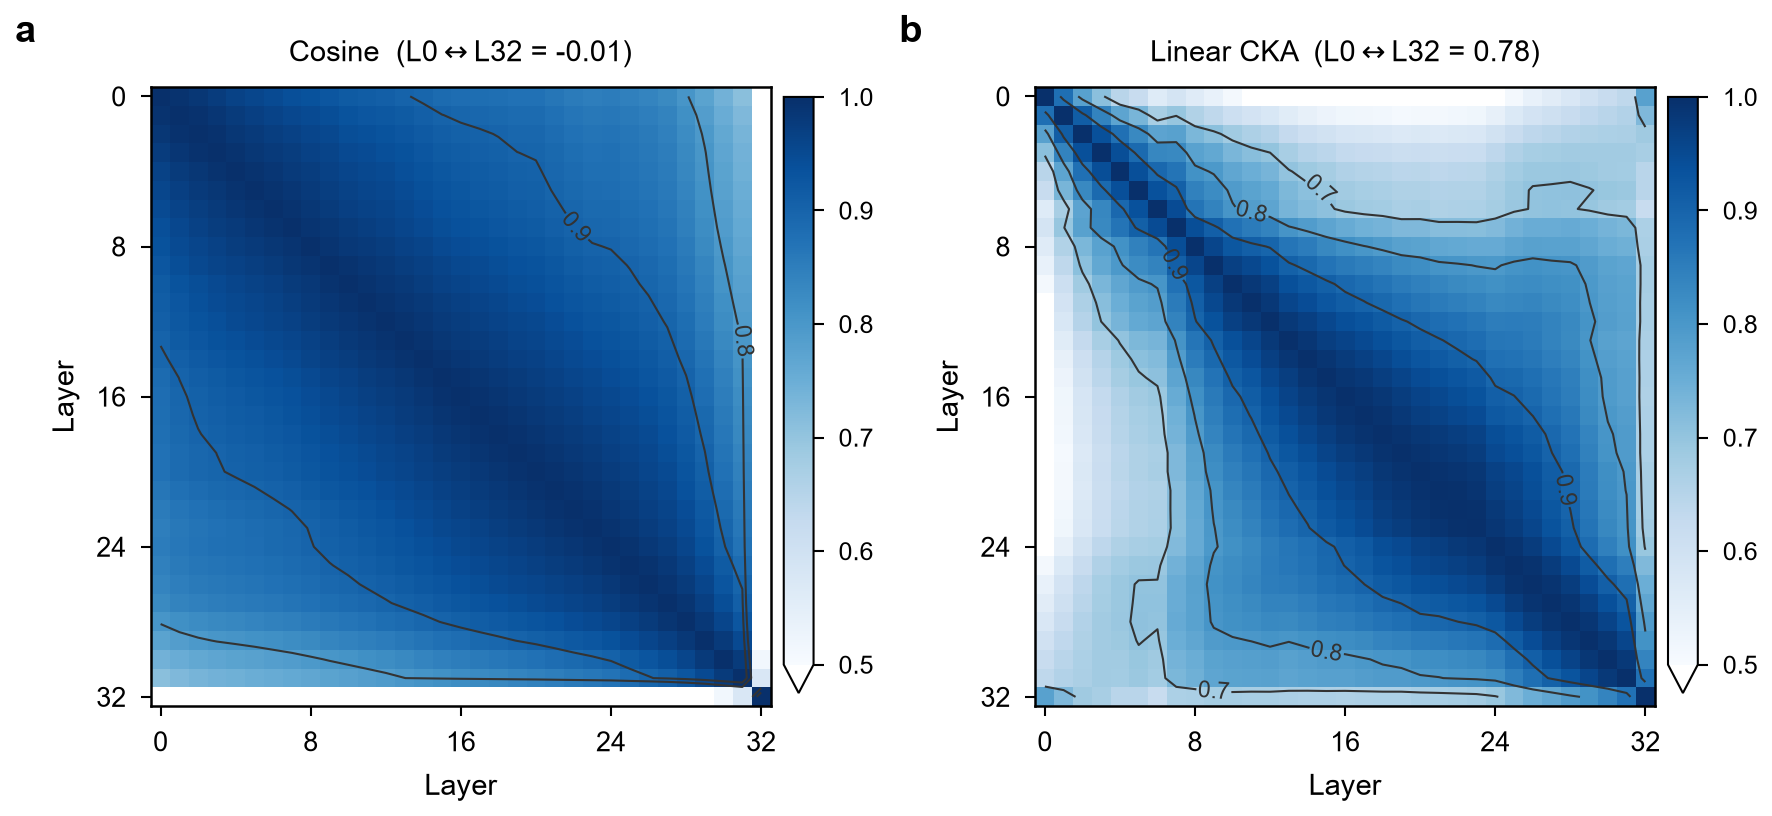
\includegraphics[width=0.7\textwidth]{figures/output_r3/fig2_similarity_heatmap.png}
\caption{\textbf{\revised{Layer-wise similarity matrices for SaProt (33$\times$33).}
Averaged over 10 datasets and \rthree{200} random residue positions per dataset.
(\textbf{a}) Cosine: adjacent layers are highly similar ($\cos=0.98$); mean similarity
decays monotonically with distance and collapses to $-0.01$ only between the most
distant layers (Layer~0 vs.~32). (\textbf{b}) Linear CKA over the same hidden states:
the most distant layers retain CKA \rthree{0.78}, indicating a rotation that preserves linearly
decodable information rather than information loss. \rtwo{Both panels share a
colour scale from 0.5 to 1 with contour lines at 0.7--0.9; cells below 0.5 (the
final-layer row and column in panel a\rthree{, and parts of the layer-0 and layer-1 rows
and columns in panel b}) are white.}}}
\label{fig:similarity}
\smallskip{\footnotesize\rthree{\textit{Alt text:} Two 33-by-33 heat maps of similarity between SaProt layers. Cosine similarity (a) stays high except between the final and first layers (about $-0.01$); linear CKA (b) remains moderately high throughout, 0.78 between layers 0 and 32.}}
\end{figure}

The matrix revealed a smooth representational trajectory across layers. Adjacent layers
were highly similar (\rthree{mean adjacent-layer cosine 0.979 for SaProt and 0.962 for
ESM-2}), and similarity \rtwo{decreased with
layer distance (Pearson $r$ over unique layer pairs: $-0.50$ for SaProt, $-0.93$ for
ESM-2)}. \revised{The decay was smooth and
monotonic, with no intermediate trough: for SaProt the mean cosine by distance fell
from 0.97 ($d=2$) through \rthree{0.81} ($d=20$) to 0.50 ($d=30$), collapsing to \rthree{$-0.008$}
between the most distant layers (Layer~0 vs.\ Layer~32). ESM-2 decayed more gently and
remained positive throughout (0.93 at $d=2$, \rthree{0.54} at $d=32$). Crucially, near-zero raw
cosine does not imply lost information: the linear CKA between SaProt layers 0 and 32
was \rthree{0.78} while their cosine was \rthree{$-0.008$ (ESM-2: CKA 0.41, cosine 0.54; adjacent-layer
CKA 0.97 for SaProt and 0.95 for ESM-2). With 50 positions per dataset the standard
estimator, which is biased upward when positions are fewer than hidden dimensions, gave
higher distant-layer values (SaProt 0.81, ESM-2 0.55); the debiased estimator is not
estimable at either sample size (Supplementary Table S3). For SaProt,} the depth-wise
transformation is therefore
well described as a rotation of the representation that \rtwo{retains much} linearly
decodable information (Figure~\ref{fig:probing}c)\rthree{; for ESM-2, the most distant
layers share less linear structure (CKA 0.41) despite a positive raw cosine}.} \rtwo{Similarity alone cannot show
whether mutation-relevant information changes with depth; we therefore measured it
directly with supervised probing, multi-scale pooling, and the logit lens.}

\subsection{\revised{Random-Split Layer Invariance Is Largely Position Memorization}}

We first asked \revised{whether the near-flat random-split layer profile reflects genuine
representational redundancy. \rtwo{Under our pipeline the profile is flat}: for the
masked\_wt arm, per-layer mean $\rho$ spans
$0.603$--$0.606$ for both models with invariance scores $\sigma \approx 5 \times
10^{-4}$ to $1.2 \times 10^{-3}$ (Table~\ref{tab:probing}). A Ridge regressor given
\emph{random vectors indexed only by mutation position} plus the same auxiliary
features recovered $\rho = 0.600$ under the random split (Table~\ref{tab:control}),
matching the full masked-position PLM probing level. Under leakage-free splits the
same control collapsed to $\rho = 0.138$ (modulo), $0.096$ (contiguous, $n=57$), and
$0.135$ (position-grouped), a paired drop of $-0.46$ (random versus modulo, Wilcoxon
$p = 5.2 \times 10^{-12}$); the random vectors alone carried $0.557$ under the random
split and approximately zero elsewhere, and the auxiliary features alone fell from
$0.339$ to $0.19$--$0.23$. Because every mutation at the same position shares one
masked-position embedding, the random-split task is solvable by a position lookup
table; the flat layer profile is therefore largely an artifact of position
memorization rather than evidence that mutation information is distributed uniformly
across depth.}

\begin{table}[ht]
\centering
\caption{\revised{Random-position lookup control (63 datasets; contiguous $n = 57$).
Mean Spearman $\rho$ of Ridge regressors given no sequence information. The control
reproduces the random-split PLM probing level and collapses under leakage-free
splits.}}
\label{tab:control}
\begin{tabular}{lcccc}
\toprule
Features & Random & Modulo & Contiguous & Position-grouped \\
\midrule
Random position vector + aux & 0.600 & 0.138 & 0.096 & 0.135 \\
Random position vector only  & 0.557 & $-0.008$ & $-0.056$ & $-0.010$ \\
Auxiliary only               & 0.339 & 0.230 & 0.188 & 0.228 \\
\bottomrule
\end{tabular}
\end{table}

\revised{Table~\ref{tab:probing} and Figure~\ref{fig:probing}a report the \rtwo{per-layer
probing} of all three arms,
both models, and all four splits ($n = 63$; contiguous $n = 57$). \rtwo{Three} patterns are
stable across every leakage-free column. \rtwo{First, performance rises substantially
with depth (Supplementary Tables \rthree{S5--S7}; Figure~\ref{fig:position_level}b): for ESM-2
masked\_wt, $\rho$ rises from 0.232 at layer 0 to 0.344 at layer 16 and 0.459 at layer
32 under the modulo split, and from 0.067 to 0.370 under the contiguous split; SaProt
with real 3Di tokens rises from 0.274 to 0.460 (masked\_wt, modulo).} \rtwo{Second}, the
best layer sits in a narrow late band: layers 30--32 are best in 26 of 27
\rtwo{leakage-free} model--arm--split combinations (layer 27 in the remaining one).
\rtwo{Third, the best layer is at most marginally better than the final layer: \rthree{the mean
per-dataset difference was at most $\Delta\rho = 0.009$ for the wild-type arms and at most
$0.019$ for the mutant arm (ESM-2, position-grouped split; 90\% upper bound $0.036$). Of
the 21 combinations in which the best layer was not the final layer, 7 were equivalent
within the $\pm 0.01$ margin, 14 were inconclusive, and none indicated a difference
beyond the margin (Supplementary Table S4). Three of the seven equivalence verdicts have
upper bounds within $0.0005$ of the margin, and the $t$-based interval and TOST each
classify one fewer comparison as equivalent, so these verdicts depend on the interval
method. Deficits of this size are small compared with the cross-dataset standard
deviation of about $0.17$.} Because these tests compare the best layer only with the
final layer, they show that the final layer is a sufficient choice, not that layers
are interchangeable.} The
invariance score rose from $\sigma \approx 10^{-3}$ (masked\_wt, random) to
$4$--$7 \times 10^{-2}$ under leakage-free evaluation, yet remained well below the
cross-dataset standard deviation ($\approx 0.17$): performance varies far more
\emph{across} datasets than \emph{across layers}, but under leakage-free evaluation
the residual layer variation has a consistent direction, favoring the final layers.
\rthree{The mutant arm exceeded the wild-type arms under the random split (ESM-2:
0.681 versus 0.606) but not under leakage-free evaluation on single substitutions. There
it was below both wild-type arms for ESM-2 (modulo, best layer: 0.443 versus 0.476 and
0.492) and level with them for SaProt with real 3Di tokens (0.492 versus 0.484 and
0.500; Supplementary Table S8). Under leakage-free evaluation, the mutant-sequence
embedding therefore did not outperform the wild-type context embedding combined with
the auxiliary substitution features.}}

\begin{table}[ht]
\centering
\caption{\revised{Unified per-layer probing, combined features (mean Spearman
$\rho$; best layer in parentheses, followed by the final-layer value when the best
layer is not layer 32). $n = 63$; contiguous $n = 57$. \rthree{Mutant-arm entries under
the leakage-free splits ($^{\dagger}$) are computed on single-substitution variants
(Section 2.2).} Full 33-layer curves in
Supplementary \rthree{Tables S5--S7}; per-dataset results in Supplementary Table \rthree{S1}.}}
\label{tab:probing}
\resizebox{\textwidth}{!}{%
\begin{tabular}{llcccc}
\toprule
Model & Arm & Random & Modulo & Contiguous & Pos.-grouped \\
\midrule
ESM-2 & masked\_wt   & 0.606 (32) & 0.459 (32) & 0.370 (32) & 0.450 (32) \\
ESM-2 & unmasked\_wt & 0.606 (32) & 0.470 (32) & 0.388 (32) & 0.461 (32) \\
ESM-2 & mutant       & 0.681 (32) & \rthree{0.443 (30) $\rightarrow$ 0.427$^{\dagger}$} & \rthree{0.353 (31) $\rightarrow$ 0.346$^{\dagger}$} & \rthree{0.444 (30) $\rightarrow$ 0.425$^{\dagger}$} \\
\midrule
SaProt (mask) & masked\_wt   & 0.603 (31) $\rightarrow$ 0.603 & 0.391 (30) $\rightarrow$ 0.386 & 0.282 (31) $\rightarrow$ 0.274 & 0.385 (31) $\rightarrow$ 0.382 \\
SaProt (mask) & unmasked\_wt & 0.604 (32) & 0.412 (30) $\rightarrow$ 0.406 & 0.324 (31) $\rightarrow$ 0.320 & 0.403 (27) $\rightarrow$ 0.400 \\
SaProt (mask) & mutant       & 0.652 (23) $\rightarrow$ 0.651 & \rthree{0.434 (30) $\rightarrow$ 0.428$^{\dagger}$} & \rthree{0.310 (30) $\rightarrow$ 0.307$^{\dagger}$} & \rthree{0.429 (30) $\rightarrow$ 0.423$^{\dagger}$} \\
\midrule
SaProt (3Di) & masked\_wt   & 0.606 (32) & 0.461 (31) $\rightarrow$ 0.460 & 0.394 (31) $\rightarrow$ 0.394 & 0.454 (31) $\rightarrow$ 0.453 \\
SaProt (3Di) & unmasked\_wt & 0.606 (27) $\rightarrow$ 0.605 & 0.473 (31) $\rightarrow$ 0.466 & 0.415 (31) $\rightarrow$ 0.406 & 0.467 (31) $\rightarrow$ 0.459 \\
SaProt (3Di) & mutant       & 0.684 (26) $\rightarrow$ 0.683 & \rthree{0.492 (30) $\rightarrow$ 0.486$^{\dagger}$} & \rthree{0.449 (31) $\rightarrow$ 0.439$^{\dagger}$} & \rthree{0.490 (31) $\rightarrow$ 0.481$^{\dagger}$} \\
\bottomrule
\end{tabular}}
\end{table}

\subsection{\revised{Multi-Scale Pooling \rthree{Does Not Reliably Improve on the Final Layer} Under a Leakage-Free Protocol}}

\revised{We ran the pooling benchmark (mutant arm, modulo
split, GCV-regularized Ridge, fold-internal standardization, attention weights trained
per fold) on the 20-dataset design subset for each model
(Table~\ref{tab:pooling}; Figure~\ref{fig:probing}b).
For SaProt (structure-masked inputs), all four strategies occupied a narrow band for
every readout (Ridge spread across strategies 0.005; LightGBM 0.014). For ESM-2,
spreads were likewise small (Ridge 0.041; LightGBM 0.050), and the best single
configuration was the last layer with LightGBM ($\rho = 0.508$), exceeding every
multi-scale strategy under every readout. Per-fold-trained attention pooling was
never the best strategy for either model. \rtwo{Paired per-dataset comparisons confirm
this (Supplementary Table \rthree{S9}): no strategy--readout combination
\rthree{significantly improved on} the last layer (largest mean difference $+0.018$, Concat~5L with Ridge, 90\%
CI $-0.008$ to $+0.044$\rthree{, which does not exclude a gain of that size}), and 14 of 24 combinations, all with nonlinear readouts, were
significantly worse (90\% CI below zero).} \rthree{Excluding the two datasets that
contain multi-site variants left this unchanged (no combination significantly better;
17 of 24 significantly worse). Under the random split, by contrast, some fusion
strategies did exceed the last layer: Concat~5L for ESM-2 with Ridge, Random Forest,
and LightGBM ($+0.009$ to $+0.012$, 90\% CIs excluding zero), and 10 of 12
strategy--readout combinations for SaProt ($+0.010$ to $+0.064$).} \rthree{The same
benchmark on the masked\_wt arm gave a similar picture (Supplementary Table S9). Under
the modulo and contiguous splits no combination significantly improved on the last
layer for ESM-2, and one did for SaProt (Concat~5L with Ridge, modulo split, $+0.020$,
90\% CI $+0.006$ to $+0.034$). Across both arms, both models, and both position-based
fold schemes, 1 of 96 strategy--readout comparisons favoured fusion and 55 favoured
the last layer; one gain among 96 intervals is fewer than expected by chance at this
interval level.}}

\begin{table}[ht]
\centering
\caption{\revised{Multi-scale pooling under the unified leakage-free pipeline (mutant
arm, modulo split, combined features; 20 datasets per model; mean $\rho \pm$ sd).
Spreads across strategies: ESM-2 Ridge 0.041, RF 0.057, MLP 0.045, LightGBM 0.050;
SaProt Ridge 0.005, RF 0.010, MLP 0.039, LightGBM 0.014. \rthree{Two of the 20 datasets
contain multi-site variants; excluding them does not change the paired comparisons
(Supplementary Table S9).}}}
\label{tab:pooling}
\begin{tabular}{lcccc}
\toprule
\textbf{ESM-2 650M} & Ridge & RF & MLP & LightGBM \\
\midrule
Last Layer (baseline) & $0.463 \pm 0.174$ & $0.476 \pm 0.173$ & $0.480 \pm 0.198$ & $\mathbf{0.508} \pm 0.189$ \\
Mean L20--33          & $0.473 \pm 0.180$ & $0.420 \pm 0.165$ & $0.436 \pm 0.179$ & $0.457 \pm 0.174$ \\
Concat 5L             & $0.481 \pm 0.183$ & $0.453 \pm 0.181$ & $0.435 \pm 0.170$ & $0.495 \pm 0.190$ \\
Attention-weighted    & $0.439 \pm 0.201$ & $0.419 \pm 0.209$ & $0.440 \pm 0.209$ & $0.463 \pm 0.208$ \\
\midrule
\textbf{SaProt\_650M\_AF2} & Ridge & RF & MLP & LightGBM \\
\midrule
Last Layer (baseline) & $0.432 \pm 0.163$ & $0.415 \pm 0.174$ & $0.445 \pm 0.168$ & $\mathbf{0.448} \pm 0.178$ \\
Mean L20--33          & $0.433 \pm 0.166$ & $0.415 \pm 0.166$ & $0.429 \pm 0.166$ & $0.439 \pm 0.182$ \\
Concat 5L             & $0.434 \pm 0.185$ & $0.407 \pm 0.173$ & $0.406 \pm 0.176$ & $0.436 \pm 0.183$ \\
Attention-weighted    & $0.429 \pm 0.164$ & $0.405 \pm 0.166$ & $0.426 \pm 0.164$ & $0.433 \pm 0.177$ \\
\bottomrule
\end{tabular}
\end{table}

\subsubsection{\rtwo{Readout Choice Matters More Than Layer Fusion for ESM-2} \rthree{Under Leakage-Free Evaluation}}

\rtwo{Pooling comparisons in which feature construction, masking state,
regularization, or split protocol differ between cells can manufacture apparent
readout-specific layer dependences much larger than any effect seen when the pipeline
is held fixed. With the pipeline held fixed, the largest single improvement for ESM-2
came from the readout rather than from fusion: on the last layer, LightGBM exceeded
Ridge by $+0.045$ under the modulo split (paired 90\% CI $+0.021$ to $+0.068$,
Wilcoxon $p = 0.011$), whereas for SaProt the contrast was not significant
($+0.016$, CI $-0.016$ to $+0.048$, $p = 0.57$; Supplementary Table \rthree{S10}).}
\rthree{The readout ranking is itself protocol-dependent: under the random split,
last-layer LightGBM was below Ridge for both models (ESM-2 $-0.035$, SaProt $-0.065$;
90\% CIs excluding zero).}

\begin{figure}[ht]
\centering
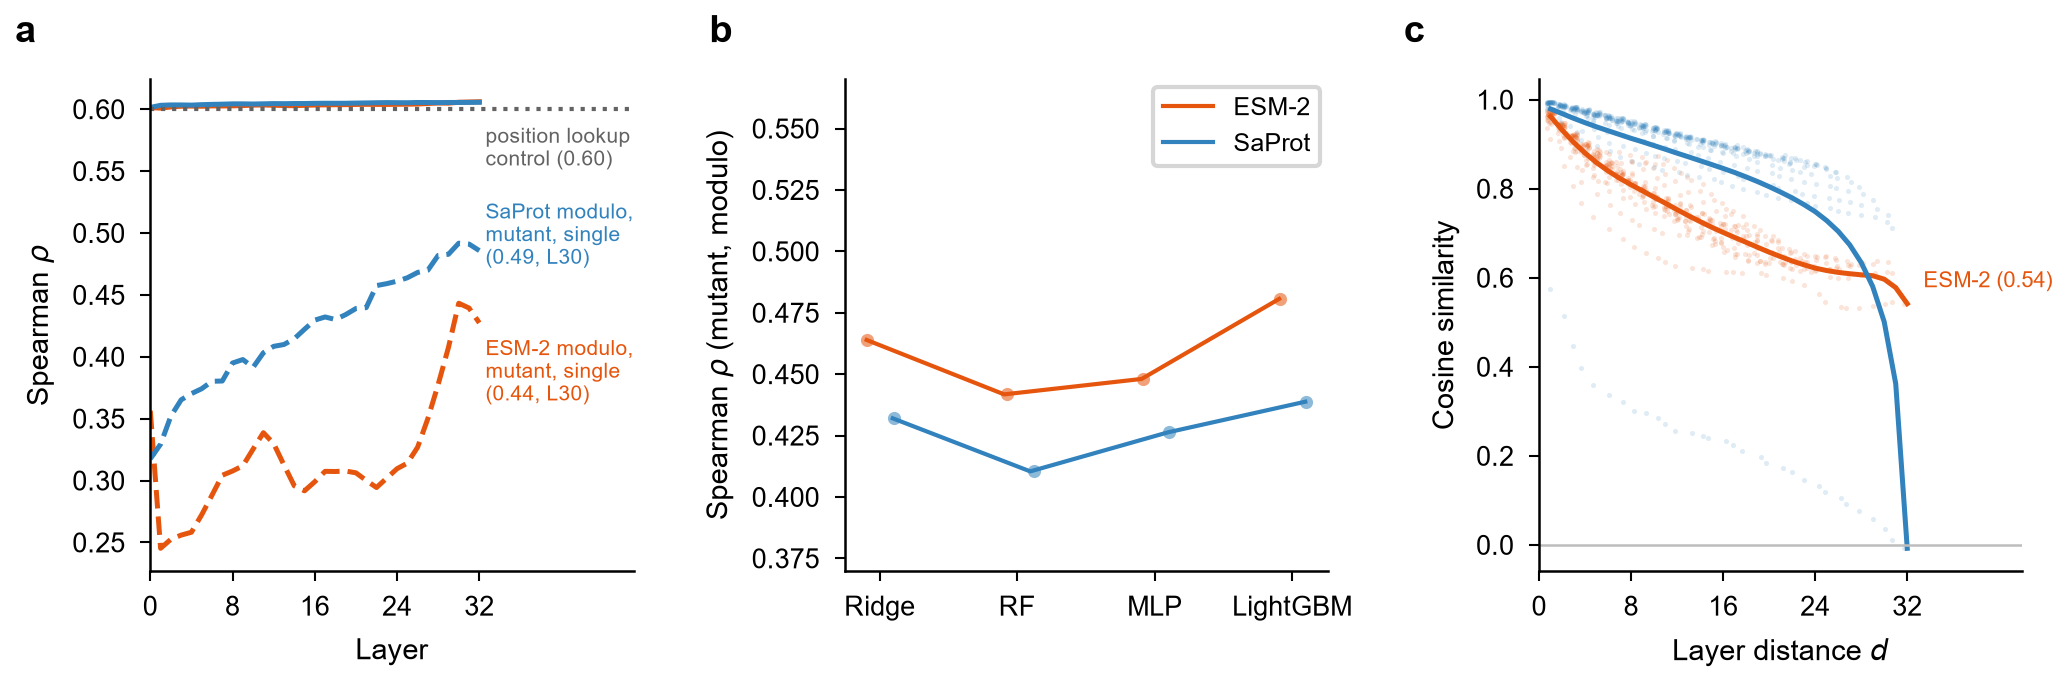
\includegraphics[width=\textwidth]{figures/output_r3/fig3_probing_pooling_summary.png}
\caption{\textbf{\revised{Per-layer probing, multi-scale pooling, and layer distance under
the unified protocol.}}
(\textbf{a}) \revised{33-layer probing (combined features): under the random split the
masked-arm profile is flat for both models ($\sigma \approx 10^{-3}$) and is reproduced by
the random-position lookup control (dotted, 0.600); under leakage-free splits (modulo,
mutant arm \rthree{on single substitutions}) performance is lower and the best layers are
\rthree{late (layer 30 for both models).}}
(\textbf{b}) \revised{Pooling (mutant arm, modulo split, 20 datasets per model; four
strategies as dots, mean connected): ESM-2 spread across strategies 0.041 (Ridge) to 0.057
(RF); SaProt spread 0.005 (Ridge) to 0.039 (MLP); last-layer LightGBM is the best single
configuration; per-fold-trained attention pooling is never best.}
(\textbf{c}) \revised{Cosine similarity versus layer distance (unique layer pairs):
SaProt decays monotonically and reaches $-0.01$ only at the largest distances, while
ESM-2 remains positive; linear CKA between the most distant SaProt layers remains \rthree{0.78}
(Figure~\ref{fig:similarity}), indicating rotation with preserved linear information
rather than loss \rthree{(200 positions per dataset)}.}}
\label{fig:probing}
\smallskip{\footnotesize\rthree{\textit{Alt text:} Three panels. (a) Under the random split, per-layer probing is flat at about 0.60 and matches the position-lookup control; under the modulo split, single-substitution mutant-arm curves are lower and peak at layer 30. (b) Pooling results by readout for both models. (c) Cosine similarity declines with layer distance.}}
\end{figure}

\subsection{Logit Lens \revised{Confirms Late-Layer Information Accumulation}}
\label{sec:lens}

\revised{The lens (fp32, per-dataset validation against the official
logits pathway, $n = 63$) produced monotonically improving zero-shot scores with
depth for both models (Figure~\ref{fig:logit_lens}). ESM-2 rose from $\rho = 0.031$
(layer 0) to $\rho = 0.443$ (layer 32), with only shallow fluctuations in early
layers; SaProt with real 3Di tokens rose from $-0.077$ (layer 0) through
approximately zero around layer 20 to $\rho = 0.437$ (layer 32). Both curves attain
their maximum at the final layer\rtwo{, in agreement with} the leakage-free probing:
mutation-relevant information accumulates toward the final layers. Zero-shot absolute
levels remain below supervised probing (0.44 versus up to \rthree{0.49}), so the lens is best
read as a consistency check on layer-wise trends rather than a standalone benchmark.}

\rtwo{To anchor these values, we recomputed published ProteinGym v1.3 per-assay results
on the 46 assays shared with our snapshot (Supplementary Table \rthree{S11}). The published
zero-shot Spearman values on these assays are 0.472 for ESM-2 650M and 0.481 for SaProt
650M; our final-layer lens gives 0.438 and 0.440, and our zero-shot reproduction of
SaProt with the authors' pipeline gives 0.484 (per-assay correlation with the published
SaProt values $r = 0.98$). On the 38 shared assays that contain only single
substitutions, the lens reproduces the published values (ESM-2 0.475 versus 0.476,
per-assay $r = 1.00$; SaProt 0.473 versus 0.477, $r = 0.97$); the remaining gap arises in
8 multi-site assays, where the lens scores each substitution of a variant separately
rather than summing over the variant. For supervised anchoring, the v1.3 release
provides out-of-fold predictions of published supervised models under its official
fold schemes. On the same 46 assays, Kermut reaches 0.605 and ProteinNPT 0.566 under
the modulo split (0.561 and 0.525 under the contiguous split), above our leakage-free
probing \rthree{on the same assays (0.24--0.47 across models and arms)}, whereas the published one-hot baseline without
augmentation falls from 0.570 under the random split to $-0.003$ under the modulo
split, an external counterpart of our position-lookup control.} \rthree{On these
assays, our final-layer mutant arm on single substitutions reaches 0.407 (ESM-2) and
0.469 (SaProt with real 3Di) under the modulo split (Supplementary Table S11).}

\begin{figure}[ht]
\centering
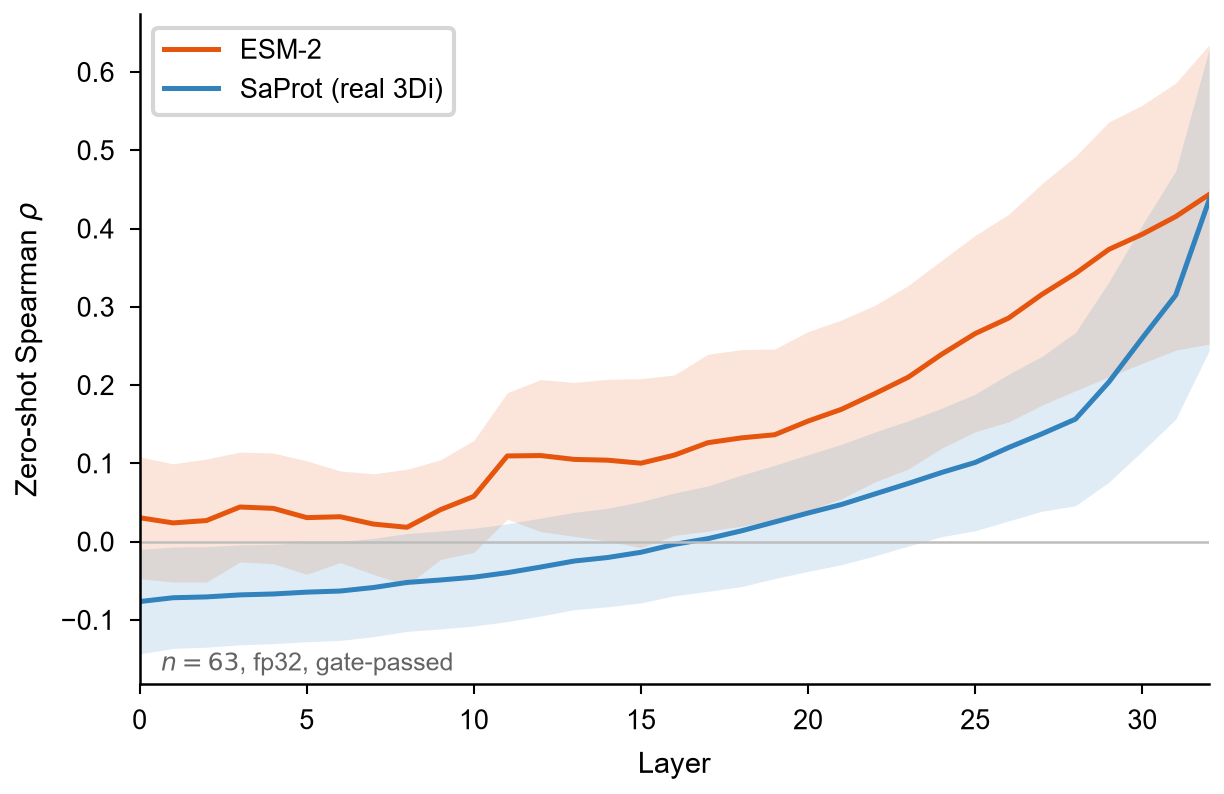
\includegraphics[width=0.85\textwidth]{figures/output_r3/fig1_logit_lens.png}
\caption{\textbf{Logit lens: zero-shot mutation scoring by layer ($n = 63$).}
\revised{Both models improve with depth and attain their maximum at the final layer:
ESM-2 (orange) rises from $\rho = 0.03$ (layer 0) to $\rho = 0.443$ (layer 32);
SaProt with real 3Di tokens (blue) rises from negative early-layer values to
$\rho = 0.437$ (layer 32). Shaded bands indicate $\pm 1$ standard deviation across
datasets. All computations in fp32 and validated against the official logits
pathway.}}
\label{fig:logit_lens}
\smallskip{\footnotesize\rthree{\textit{Alt text:} Line plot of zero-shot logit-lens Spearman correlation against layer for ESM-2 and SaProt; both curves rise with depth and peak at the final layer at about 0.44.}}
\end{figure}

\subsection{Boundary Conditions}
\label{sec:boundary}

\rtwo{The results above show that what a benchmark reports about layer choice depends
on how it is evaluated. We now examine the two factors that moderate every
conclusion: evaluation protocol and input representation.}

\subsubsection{\revised{Leakage-Free Splits: What Is Lost and What Remains}}

\revised{The control and main-table results above already localize the leakage: the
random-position lookup table reproduces the random-split level ($0.600$ versus
$0.603$--$0.606$ for full probing) and loses it entirely under leakage-free splits
($0.10$--$0.14$), while the random vectors alone carry $0.557$ under the random
split and approximately zero elsewhere (Tables~\ref{tab:control}
and~\ref{tab:probing}; Figure~\ref{fig:position_level}). Among the leakage-free
splits, modulo and position-grouped give similar levels (e.g., SaProt real-3Di
\rthree{unmasked\_wt arm: $0.473$ and $0.467$}) while contiguous is uniformly hardest (\rthree{$0.415$}),
consistent with sequence-contiguous segments correlating with local structural
context and mutational scope. Random mutation splitting, the de facto standard in DMS
benchmarking, therefore inflates \rthree{final-layer} performance estimates by
\rthree{$0.14$--$0.26$ $\rho$ relative to the modulo and position-grouped splits and by
$0.20$--$0.34$ relative to the contiguous split} and masks both layer differences and
structure-token contributions. \rtwo{ProteinGym already provides the modulo and
contiguous schemes used here~\cite{notin2024proteingym}; results under the random split
alone overstate performance and conceal the depth trend, a situation analogous to
random versus temporal cross-validation for time series~\cite{roberts2017crossvalidation}.}}

\subsubsection{\rtwo{Multi-Site Variants \rthree{and Single-Substitution Analysis}}}

\rtwo{Because the position-based splits assign each row by its own substitution
position, rows of the same multi-site variant can share a fitness label across folds\rthree{.
In the mutant arm they also share the variant's averaged embedding. Under the modulo
split, 15,624 of the 213,393 analyzed rows (7.3\%) are test rows whose variant also has
a row in the training folds (15,960 under the position-grouped split and 6,158 under
the contiguous split). Re-running all three arms on single-substitution variants only
(Supplementary Table S8) shows that this inflated the full-data mutant arm (ESM-2,
modulo, best layer: 0.483 on the full data versus 0.443 on single substitutions;
SaProt with real 3Di: 0.531 versus 0.492). It did not inflate the wild-type arms (ESM-2
masked\_wt: 0.459 versus 0.476), so only the mutant arm is analyzed on single
substitutions under these splits. On single substitutions the depth trend and the late
optimum were unchanged for all arms, with the best layer in layers 27--32 in every
leakage-free column. The best layer exceeded the final layer by at most 0.019 (point
estimates; 90\% upper bounds up to 0.036; 3 of 23 comparisons equivalent, 20
inconclusive, none beyond the margin). Two datasets retain fewer than 50 single-substitution variants;
excluding them leaves these conclusions unchanged (largest point estimate 0.014, 90\%
upper bound 0.025).}}

\begin{figure}[ht]
\centering
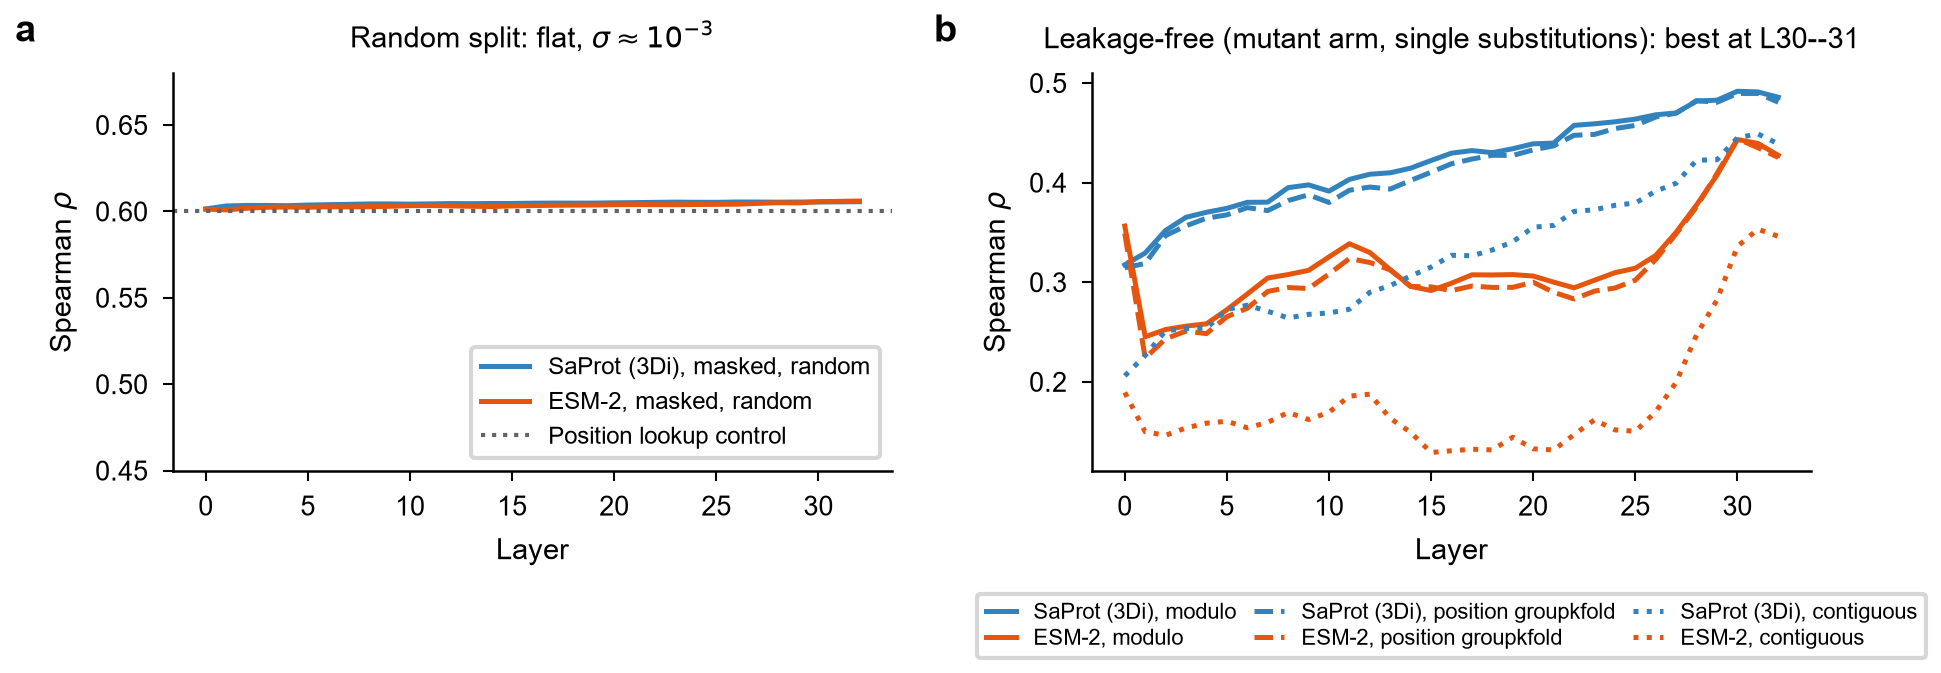
\includegraphics[width=\textwidth]{figures/output_r3/fig5_position_level.png}
\caption{\textbf{\revised{Random versus leakage-free split probing (\rthree{ESM-2 and SaProt}, 63 datasets).}}
(\textbf{a}) \revised{Random mutation split: flat per-layer profile
($\sigma \approx 10^{-3}$), reproduced by the random-position lookup control
($\rho = 0.600$).} (\textbf{b})
\revised{Leakage-free splits (modulo, position-grouped, contiguous\rthree{; mutant arm on
single substitutions}): performance
drops to \rthree{$0.35$--$0.49$}, the invariance score rises to
$4$--$7 \times 10^{-2}$, and the best layers shift consistently to layers \rthree{30--31}.}}
\label{fig:position_level}
\smallskip{\footnotesize\rthree{\textit{Alt text:} Two panels of per-layer probing for ESM-2 and SaProt. (a) Under the random split, curves are flat at about 0.60 and match the position-lookup control. (b) Under leakage-free splits, single-substitution mutant-arm curves are lower (0.35 to 0.49) and peak at layers 30 to 31.}}
\end{figure}

\revised{Together, these boundary conditions refine the central finding: apparent
layer \rtwo{interchangeability} under random splitting is dominated by position
memorization, leakage-free evaluation reveals \rtwo{a consistent depth trend in which
the final layer is sufficient}, and the benefit of structure tokens \rtwo{depends
strongly on} the evaluation protocol.}

\subsection{\revised{Structure Tokens Help \rtwo{Most} Under Leakage-Free Evaluation}}

\revised{Because SaProt can be run with real 3Di tokens or with structure-masked
tokens, the unified protocol allows a paired test, dataset by dataset and layer by
layer, of what structure tokens actually contribute (Table~\ref{tab:3di}). Under the
random split the \rtwo{differences were small} (paired differences at layer
32: $+0.003$ masked\_wt, $+0.002$ unmasked\_wt, $+0.032$ mutant\rtwo{; Wilcoxon
$p = 0.022$, $0.91$, and $2.5 \times 10^{-6}$, so the effect is small but clearly
non-zero for the mutant arm}). Under every
leakage-free split the real-3Di inputs were consistently superior, with mean paired
advantages of \rthree{$+0.057$ to $+0.132$} across arms and splits, all with Wilcoxon
\rthree{$p \leq 0.0011$ (mutant arm on single substitutions)}. Structure tokens therefore carry genuine mutation-relevant
information\rtwo{; the contribution is small under random splitting and becomes large
once position memorization is removed from the evaluation, consistent with the
position channel, available to both input modes, saturating most of the random-split
task.}}

\begin{table}[ht]
\centering
\caption{\revised{Real-3Di versus structure-masked SaProt inputs (paired per-dataset
differences at layer 32, combined features; Wilcoxon signed-rank $p$). The benefit of
structure tokens is small under the random split \rtwo{(significant for the masked\_wt
and mutant arms)} and large and highly significant under all leakage-free splits.
\rthree{Mutant-arm entries under the leakage-free splits ($^{\dagger}$) are computed on
single-substitution variants.}}}
\label{tab:3di}
\resizebox{\textwidth}{!}{%
\begin{tabular}{lcc|ccc}
\toprule
& \multicolumn{2}{c|}{\textbf{Random}} & \multicolumn{3}{c}{\textbf{Leakage-free}} \\
Arm & $\Delta\rho$ & $p$ & Modulo & Contiguous & Pos.-grouped \\
\midrule
masked\_wt   & $+0.003$ & $2.2 \times 10^{-2}$ & $+0.073$ ($3.5 \times 10^{-7}$) & $+0.120$ ($8.7 \times 10^{-8}$) & $+0.071$ ($8.4 \times 10^{-7}$) \\
unmasked\_wt & $+0.002$ & $9.1 \times 10^{-1}$ & $+0.060$ ($4.6 \times 10^{-6}$) & $+0.086$ ($2.1 \times 10^{-6}$) & $+0.059$ ($1.2 \times 10^{-5}$) \\
mutant       & $+0.032$ & $2.5 \times 10^{-6}$ & \rthree{$+0.057$ ($1.0 \times 10^{-3}$)$^{\dagger}$} & \rthree{$+0.132$ ($4.8 \times 10^{-7}$)$^{\dagger}$} & \rthree{$+0.058$ ($1.1 \times 10^{-3}$)$^{\dagger}$} \\
\bottomrule
\end{tabular}}
\end{table}

%=============================================================================
\section{Discussion}
%=============================================================================

\rtwo{The central result of this study has two parts. Under the standard random-split
protocol, the 33 transformer layers of SaProt and ESM-2 show near-flat mutation effect
prediction performance, but the position-lookup control shows that this flatness is
largely position memorization, a property of the evaluation rather than of the
representations. Under leakage-free evaluation, performance rises substantially with
depth, the best layers are the last few (layers 27--32), the final layer is within
\rthree{$\Delta\rho = 0.019$ of the best layer (point estimates; 90\% upper bounds up to
0.036)}, and structure tokens deliver a measurable benefit (\rthree{$+0.06$ to $+0.13$}).
\rthree{Multi-scale pooling did not reliably improve on the final layer under leakage-free
evaluation (1 of 96 comparisons significantly better).} The practical conclusion is therefore not that multi-scale embeddings are
never useful, but that for mutation effect prediction with these 650M models depth
matters and the final layer is a sufficient choice.}

\subsection{\rtwo{Why Does Performance Increase With Depth?}}

\rtwo{We propose that the depth trend reflects the MLM pre-training objective. All
layers receive gradients through the same cross-entropy loss computed at the final LM
head, so successive layers are optimized to move representations toward the
conditional amino-acid distributions that the LM head predicts---the quantities that
a mutation-effect readout ultimately uses. Mutation-relevant signal therefore
accumulates with depth rather than being distributed across specialized layers, and
the last layers carry most of it. Under random-split evaluation this trend is hidden
because position memorization dominates the task.}

\revised{The cosine similarity between layers decays monotonically with distance and,
for SaProt, collapses to approximately zero only between the most distant layers,
while the linear CKA between the same layers remains \rthree{0.78}. This combination, a
near-rotation that preserves linearly decodable information, is consistent with the
effect of residual connections~\cite{he2016deep}: because residual streams accumulate
representations from all preceding layers, late layers retain a linearly accessible
trace of early-layer content even as their raw coordinates rotate.}

This interpretation is consistent with the logit lens
hypothesis~\cite{nostalgebraist2020,belrose2023eliciting},
which posits that intermediate layers in transformer language models progressively
refine token predictions toward the final output distribution, rather than
constructing qualitatively different representations. \revised{The lens
curves support this directly for both models: zero-shot scoring improves with depth
and peaks at the final layer.} The near-orthogonality of the most distant SaProt
layers ($\cos \approx -0.01$) \revised{alongside their high linear CKA (\rthree{0.78})}
\rtwo{suggests that linearly decodable information is retained while representations
move through successive coordinate frames, even as mutation-relevant signal continues
to accumulate.}

\rthree{In NLP transformers, by contrast, probing classifiers recover different
linguistic features at different depths~\cite{tenney2019bert,rogers2021bertology}. The
comparison is limited: we probe a single prediction target, which would be expected to
give one peaked curve, whereas NLP studies probe many distinct features, and early PLM
layers are known to encode local physicochemical and secondary-structure
properties~\cite{detlefsen2022}. Whether PLM layers specialize less than NLP layers is
therefore a hypothesis that would require probing several distinct protein properties
under leakage-free splits.}

\subsubsection{\revised{What Separates SaProt from Standard ESM-2?}}

\revised{Under \rtwo{a single fixed} protocol the two models differ mainly in two measured
ways: how much their final representations retain early-layer geometry (ESM-2
distant-layer cosine \rthree{0.54 with CKA 0.41}; SaProt cosine $-0.01$ with CKA \rthree{0.78}), and the benefit conferred by structure tokens. The directly measured
difference is the structure-token benefit: real 3Di inputs improve leakage-free
probing by \rthree{$+0.06$ to $+0.13$} while \rtwo{changing random-split performance only
slightly}. Structure information is genuinely present and genuinely useful, but
\rtwo{leakage-free evaluation is needed to measure it}.}

\revised{This framing carries a testable prediction: fine-tuning standard ESM-2
with structural objectives (e.g., contact prediction or fold classification)
should reproduce a similar leakage-free advantage over the sequence-only baseline.
This remains a mechanistic hypothesis rather than a direct result of the present
experiments.}

\subsection{Reconciling with Prior Layer-Selection Studies}

Our findings do not contradict the observation that different layers may be
optimal for different \emph{task types}. Kumar and Jha~\cite{kumar2025}
demonstrated that mid-to-late ESM-2 layers (20--33) outperform the final layer
for kinase function prediction, achieving 32\% higher clustering quality and
superior classification accuracy. \rthree{Our leakage-free results are broadly in line with this observation: for
mutation effect prediction the best layers lie in layers 27--32 and the late layers are
close to the final layer, consistent with the finding that layers 20--33 perform well.
The difference is one of degree: for kinase function prediction, intermediate layers
outperformed the final layer, whereas for mutation effect prediction the final layer is
within a small margin of the best layer. The flat random-split profile is a property of
the evaluation and is not informative for such comparisons.}

Similarly, the 12\% Spearman improvement reported by Alsamkary, Elshaffei
et al.~\cite{elshaffei2025} for attention-based fusion architectures was
observed in the context of multi-chain protein--protein interaction prediction,
a task that differs substantially from per-residue mutation effect scoring.
The benefit of sophisticated pooling may therefore be task-dependent rather than
inherent to multi-scale representation fusion. For mutation effect prediction,
our results suggest that such improvements should be interpreted in light of
model type, readout choice, and split protocol.

\subsection{Practical Implications}

\rtwo{For researchers using protein language model embeddings for mutation effect
prediction, our results support a single default for both model types: extract the
final layer. Multi-scale fusion \rthree{did not reliably improve on} the final layer for either
model under leakage-free evaluation \rthree{(one significant gain in 96 comparisons)}, and 1280 dimensions sufficed for both linear and
nonlinear readouts; this reduces storage and computational costs by a factor of 5--10
compared with concatenating 6--8 layers (up to 10,240 dimensions). Where additional
effort is available, it is better spent on the readout than on fusion, at least for
the sequence-only model: for ESM-2, last-layer LightGBM exceeded last-layer Ridge by
$+0.045$ (paired, $p = 0.011$) and reached $\rho = 0.508$, the best pooling
configuration overall, whereas for SaProt the same contrast was not significant\rthree{;
this ranking holds under the modulo split and reverses under the random split}.}

Table~\ref{tab:cost} quantifies the practical trade-offs. Concat~5L uses
$4.9\times$ more features than single-layer approaches \rtwo{and its Ridge covariance
matrix has $24\times$ more entries ($1{,}322^2$ versus $6{,}442^2$). We did not time
readout fitting separately from embedding extraction: the end-to-end time per dataset
is dominated by extraction, which requires one forward pass with all 33 layers
collected for every strategy, and is therefore similar across strategies.} Concat~5L
offered no \rthree{significant} benefit on
\revised{either model} in our \rthree{mutant-arm} benchmark \revised{and was matched or exceeded on
ESM-2 by switching from Ridge to LightGBM on a single layer}. Storing Concat~5L embeddings for a typical DMS
benchmark ($\sim$10,000 variants) requires 258~MB versus 53~MB for a single
layer, a gap that widens linearly with dataset size and becomes substantial
for genome-scale studies.

\begin{table}[ht]
\centering
\caption{Computational cost comparison across pooling strategies.
``Per-mutation'' storage assumes float32 precision. Time estimates are
per-dataset averages on an NVIDIA RTX 5090, including embedding extraction
and readout training across 20 ProteinGym DMS subsets \rtwo{(end-to-end; extraction
dominates and is identical across strategies)}.
\revised{Best achievable $\rho$ from Table~\ref{tab:pooling} (mutant arm,
modulo split).}}
\label{tab:cost}
\resizebox{\textwidth}{!}{%
\begin{tabular}{lcccc}
\toprule
& Last Layer & Mean L20--33 & Attention & Concat 5L \\
\midrule
Feature dimension                  & 1,322 & 1,322 & 1,322 & 6,442 \\
Storage per mutation (KB)          & 5.2   & 5.2   & 5.2   & 25.2 \\
Ridge design matrix (5,000 vars)   & $6.6 \times 10^6$ & same & same & $3.2 \times 10^7$ \\
Ridge covariance matrix entries    & $1.7 \times 10^6$ & same & same & $4.1 \times 10^7$ \\
Avg.\ time per dataset (min)       & $\sim$3 & $\sim$3 & $\sim$3 & $\sim$3 \\
\midrule
\multicolumn{5}{l}{\small \textbf{Best achievable $\rho$ (ESM-2 / SaProt):}} \\
\quad With Ridge                    & \revised{0.463 / 0.432} & \revised{0.473 / 0.433} & \revised{0.439 / 0.429} & \revised{0.481 / 0.434} \\
\quad With LightGBM                 & \textbf{\revised{0.508 / 0.448}} & \revised{0.457 / 0.439} & \revised{0.463 / 0.433} & \revised{0.495 / 0.436} \\
\bottomrule
\end{tabular}}
\end{table}

\rtwo{Beyond the choice of layer}, computational resources may be better directed toward feature types
that are plausibly complementary to PLM embeddings:
\begin{enumerate}
    \item Structural features (e.g., AlphaFold-predicted pLDDT, PAE~\cite{jumper2021alphafold},
          or Foldseek 3Di states~\cite{vankempen2024foldseek}), which complement
          sequence-based embeddings;
    \item Sequence-level representations that capture global protein properties
          beyond per-residue features;
    \item Multiple sequence alignment (MSA)-based approaches~\cite{riesselman2018deepsequence,
          hopf2017mutation} that leverage evolutionary information beyond what PLMs encode.
\end{enumerate}

As discussed under Boundary Conditions (Section~\rtwo{\ref{sec:boundary}}), \revised{the position-lookup
control shows that} standard evaluation protocols can conflate mutation-effect learning with
position-level memorization\rtwo{; random-split results alone therefore overstate
performance and conceal the depth trend, whereas ProteinGym's position-based splits
expose both}.

\subsection{Limitations}

Several limitations should be noted. First, we tested the 650M-parameter
ESM-2 variant and its structure-aware derivative SaProt. Smaller (35M, 150M)
and larger (3B, 15B) variants may show different degrees of layer specialization,
and this remains to be tested. Second, our
experiments are restricted to per-residue mutation effect prediction; for other
tasks such as kinase function prediction~\cite{kumar2025}, subcellular
localization, or protein--protein interaction scoring~\cite{elshaffei2025},
layer-wise differences and the benefits of multi-scale fusion may be more
pronounced. Third, our pooling benchmark used a 20-dataset validation subset,
which is smaller than the \revised{63}-dataset probing analysis. \revised{Fourth,
the SaProt pooling runs use structure-masked inputs, whereas the probing and logit
lens runs include real 3Di inputs, and one dataset (influenza nucleoprotein) lacks
an AFDB structure. Fifth, our}
feature ablation (embedding-only vs.\ auxiliary-only) indicates that learned embeddings
dominate predictive performance in this setting, but it does
not rule out the possibility that nonlinear combinations of auxiliary features
could provide stronger baselines.
\revised{Sixth,} the
maximum sample size of 10,000 \rtwo{variants} per dataset (subsampled to 5,000
\rtwo{rows} for regression\revised{; \rtwo{11 of 63 datasets were variant-capped and 26
reached the row ceiling}}) may limit sensitivity to
subtle layer-wise effects on the largest DMS screens ($>$200,000 mutations). \revised{Seventh,} our linear probing approach can only detect
information that is linearly separable; nonlinear interactions between layers
could theoretically exist but would require a different experimental design to
identify. \revised{Eighth}, position-level data splitting (Section~\rtwo{\ref{sec:boundary}}) shows that
random mutation splits permit position-level leakage, \revised{which the lookup
control quantifies and which motivates our reporting of leakage-free splits
throughout}\rtwo{\rthree{. Ninth, under the position-based splits the mutant arm is analyzed on
single substitutions, which excludes most variants of the ten datasets that contain
multi-site variants; the wild-type arms are reported on the full data, in which rows of
a multi-site variant share labels across folds, although their single-substitution
results are similar (Supplementary Table S8)}. Finally, our
equivalence margin ($\Delta\rho = 0.01$) was fixed before the equivalence analysis as
a practical convention rather than a task-derived threshold, and because the best
layer is selected on the same data, the equivalence verdicts are conservative\rthree{;
three of the seven equivalence verdicts nevertheless lie at the margin and depend on
the interval method}.}

\subsection{Conclusion}

\rtwo{For mutation effect prediction with 650M protein language models, depth
matters: under leakage-free evaluation, predictive performance rises with depth and the
best layers are the last few. The final layer is a sufficient choice---within
\rthree{$\Delta\rho = 0.019$ of the best layer (point estimates; 90\% upper bounds up to
0.036), a small deficit relative to the variation across datasets}---and \rthree{multi-scale
pooling did not reliably improve on it} under leakage-free
evaluation. Under the standard random split, by contrast, near-flat layer profiles are
reproduced by a position lookup table with no sequence information, so random-split
layer interchangeability is a property of the evaluation, not of the representations.
Structure tokens add a benefit that is small under random splitting and large under
leakage-free evaluation. These findings support extracting the final layer, evaluating
with a position-aware split, and treating claims of layer-specific representations in
PLMs with the same scrutiny that has become standard in the NLP
community~\cite{rogers2021bertology}.}

%=============================================================================
\section*{Acknowledgments}
We thank the International
College of Pharmaceutical Innovation, SUDA-RCSI for institutional support.

\section*{Funding}
\revised{This work was supported by the Jiangsu Tepin Foundation (Z241922) and
the Health Research Board (ILP-PHR-2024-014).}

\section*{Competing Interests}
\revised{The authors declare no competing interests.}

\section*{Data Availability}
Code and results are available at \url{https://github.com/schwarzeteeguo-creator/esm2-layer-invariance}.
\revised{An archived snapshot of the code, per-dataset results, and extracted
structure tokens for this revision is deposited at Zenodo (concept DOI
10.5281/zenodo.22844290; archived version \rthree{v3.1.1, DOI 10.5281/zenodo.23878920}).}
Raw ProteinGym data: \url{https://github.com/OATML-Markslab/ProteinGym}.

\newpage
\begin{thebibliography}{99}

% === References numbered by order of first citation in the text ===

\bibitem{rives2021biological}
Rives, A.\ \textit{et al.} (2021)
Biological structure and function emerge from scaling unsupervised learning to 250
million protein sequences.
\textit{Proceedings of the National Academy of Sciences}, \textbf{118}(15), e2016239118.

\bibitem{meier2021language}
Meier, J.\ \textit{et al.} (2021)
Language models enable zero-shot prediction of the effects of mutations on protein
function.
\textit{Advances in Neural Information Processing Systems}, \textbf{34}, 29287--29303.

\bibitem{lin2023evolutionary}
Lin, Z.\ \textit{et al.} (2023)
Evolutionary-scale prediction of atomic-level protein structure with a language model.
\textit{Science}, \textbf{379}(6637), 1123--1130.

\bibitem{frazer2021disease}
Frazer, J.\ \textit{et al.} (2021)
Disease variant prediction with deep generative models of evolutionary data.
\textit{Nature}, \textbf{599}(7883), 91--95.

\bibitem{hie2021learning}
Hie, B.\ \textit{et al.} (2021)
Learning the language of viral evolution and escape.
\textit{Science}, \textbf{371}(6526), 284--288.

\bibitem{elnaggar2022prottrans}
Elnaggar, A.\ \textit{et al.} (2022)
ProtTrans: Toward understanding the language of life through self-supervised learning.
\textit{IEEE Transactions on Pattern Analysis and Machine Intelligence}, \textbf{44}(10),
7112--7127.

\bibitem{brandes2022proteinbert}
Brandes, N.\ \textit{et al.} (2022)
ProteinBERT: A universal deep-learning model of protein sequence and function.
\textit{Bioinformatics}, \textbf{38}(8), 2102--2110.

\bibitem{rogers2021bertology}
Rogers, A., Kovaleva, O.\ and Rumshisky, A. (\revised{2020})
A primer in BERTology: What we know about how BERT works.
\textit{Transactions of the Association for Computational Linguistics}, \textbf{8},
842--866.

\bibitem{tenney2019bert}
Tenney, I., Das, D.\ and Pavlick, E. (2019)
BERT rediscovers the classical NLP pipeline.
\textit{Proceedings of the 57th Annual Meeting of the Association for Computational
Linguistics}, 4593--4601.

\bibitem{nostalgebraist2020}
nostalgebraist (2020)
Interpreting GPT: the logit lens.
\url{https://www.lesswrong.com/posts/AcKRB8wDpdaN6v6ru/}.

\bibitem{kumar2025}
Kumar, A.\ and Jha, I.P. (2025)
Layer probing improves kinase functional prediction with protein language models.
\textit{arXiv}, 2512.00376.

\bibitem{detlefsen2022}
Detlefsen, N.S.\ \textit{et al.} (2022)
Learning meaningful representations of protein sequences.
\textit{Nature Communications}, \textbf{13}(1), 1914.

\bibitem{elshaffei2025}
Alsamkary, H., Elshaffei, M.\ \textit{et al.} (2025)
Beyond simple concatenation: Fairly assessing PLM architectures for multi-chain
protein--protein interactions prediction.
\textit{arXiv}, 2505.20036.

\bibitem{rao2019tape}
Rao, R.\ \textit{et al.} (2019)
Evaluating protein transfer learning with TAPE.
\textit{Advances in Neural Information Processing Systems}, \textbf{32}.

\bibitem{notin2024proteingym}
Notin, P.\ \textit{et al.} (2024)
ProteinGym: Large-scale benchmarks for protein fitness prediction and design.
\textit{Advances in Neural Information Processing Systems}, \textbf{36}.

\bibitem{su2024saprot}
Su, J.\ \textit{et al.} (2024)
SaProt: Protein language modeling with structure-aware vocabulary.
\textit{International Conference on Learning Representations (ICLR)}.

\bibitem{vankempen2024foldseek}
van Kempen, M.\ \textit{et al.} (2024)
Fast and accurate protein structure search with Foldseek.
\textit{Nature Biotechnology}, \textbf{42}(2), 243--246.

\bibitem{roberts2017crossvalidation}
Roberts, D.R.\ \textit{et al.} (2017)
Cross-validation strategies for data with temporal, spatial, hierarchical, or
phylogenetic structure.
\textit{Ecography}, \textbf{40}(8), 913--929.

\bibitem{he2016deep}
He, K.\ \textit{et al.} (2016)
Deep residual learning for image recognition.
\textit{Proceedings of the IEEE Conference on Computer Vision and Pattern Recognition (CVPR)},
770--778.

\bibitem{jumper2021alphafold}
Jumper, J.\ \textit{et al.} (2021)
Highly accurate protein structure prediction with AlphaFold.
\textit{Nature}, \textbf{596}(7873), 583--589.

\bibitem{riesselman2018deepsequence}
Riesselman, A.J., Ingraham, J.B.\ and Marks, D.S. (2018)
Deep generative models of genetic variation capture the effects of mutations.
\textit{Nature Methods}, \textbf{15}(10), 816--822.

\bibitem{hopf2017mutation}
Hopf, T.A.\ \textit{et al.} (2017)
Mutation effects predicted from sequence co-variation.
\textit{Nature Biotechnology}, \textbf{35}(2), 128--135.

\bibitem{golub1979generalized}
\revised{Golub, G.H., Heath, M.\ and Wahba, G. (1979)
Generalized cross-validation as a method for choosing a good ridge parameter.
\textit{Technometrics}, \textbf{21}(2), 215--223.}

\bibitem{kornblith2019similarity}
\revised{Kornblith, S., Norouzi, M., Lee, H.\ and Hinton, G. (2019)
Similarity of neural network representations revisited.
\textit{Proceedings of the 36th International Conference on Machine Learning},
3519--3529.}

\bibitem{belrose2023eliciting}
\revised{Belrose, N. \textit{et al.} (2023)
Eliciting latent predictions from transformers with the tuned lens.
\textit{arXiv}, 2303.08112.}

\bibitem{ko2026fusion}
\rtwo{Ko, Y.S., Parkinson, J.\ and Wang, W. (2026)
Scalable embedding fusion with protein language models: insights from
benchmarking text-integrated representations.
\textit{Briefings in Bioinformatics}, \textbf{27}(1), bbag014.}

\bibitem{si2024contact}
\rtwo{Si, Y.\ and Yan, C. (2024)
Protein language model-embedded geometric graphs power inter-protein contact
prediction.
\textit{eLife}, \textbf{12}, RP92184.}

\bibitem{song2012feature}
\rtwo{Song, L., Smola, A., Gretton, A., Bedo, J.\ and Borgwardt, K. (2012)
Feature selection via dependence maximization.
\textit{Journal of Machine Learning Research}, \textbf{13}, 1393--1434.}

\end{thebibliography}

\end{document}
